%-------------------------------------------------------------------------------
\subsubsection{Modèle de Allee}
%-------------------------------------------------------------------------------

% Voir examen SU L2bio 2024-25

On considère une version canonique du modèle de dynamique de population proposé par W.C. Allee en 1949. En notant $x(t)$ la taille d'une population au temps $t$, ce modèle pose que 
\begin{equation} \label{eq:modAllee}
  \dot x = f(x) = x (x-1) (2-x).
\end{equation}

\bigskip 
\paragraph{\'Etude des points stationnaires.}
\begin{enumerate}
  \item Déterminer les trois points stationnaires $x_1^* < x_2^* < x_3^*$ du système et étudier leur stabilité.
  \solution{
    $f(x)$ s'annule pour $x_1^* = 0$, $x_2^* =1$ et $x_3^* = 2$. \\
    Concernant leur stabilité, puisque $f(x) = -x^3 + 3x^2 - 2x$, on a $f'(x) = -3x^2 + 6x - 2$ et donc
    \begin{align*}
      f'(x_1^* = 0) & = -2 < 0 : & & \text{$x_1^*$ est un équilibre stable;} \\
      f'(x_2^* = 1) & = + 1 > 0 : & & \text{$x_2^*$ est un équilibre instable;} \\
      f'(x_3^* = 2) & = -8 < 0  :& & \text{$x_3^*$ est un équilibre stable.}
    \end{align*}
  }
  \item Tracer le diagramme de stabilité et donner l'allure des solutions du système \eqref{eq:modAllee}.
  \solution{
  Le diagramme de stabilité est donc le suivant
  $$
  \begin{tikzpicture}
    \node[] (x0) at (-1*\edgeunit, 0) {}; 
    \node[] (x01) at (-0.5*\edgeunit, 0) {}; 
    \node[] (x1) at (0*\edgeunit, 0) {$x_1^*$}; 
    \node[] (x12) at (0.5*\edgeunit, 0) {}; 
    \node[] (x2) at (1*\edgeunit, 0) {$x_2^*$}; 
    \node[] (x23) at (1.5*\edgeunit, 0) {}; 
    \node[] (x3) at (2*\edgeunit, 0) {$x_3^*$}; 
    \node[] (x34) at (2.5*\edgeunit, 0) {}; 
    \node[] (x4) at (3*\edgeunit, 0) {}; 
    
    \draw[->, opacity=1] (x01) -- (x1); \draw[->] (x12) -- (x1);  
    \draw[->] (x2) -- (x12); \draw[->] (x2) -- (x23); 
    \draw[->] (x23) -- (x3); \draw[->] (x34) -- (x3);  
    \draw[lightedge, opacity=0.5] (x0) -- (x4);
  \end{tikzpicture}
  $$
  et, partant d'une taille de population initiale $x(0) > 0$, les solutions ont les allures suivantes :
  $$
  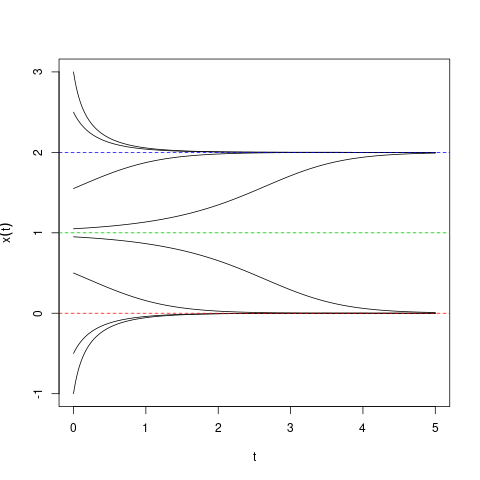
\includegraphics[width=0.5\textwidth, trim=0 10 20 50, clip=]{Allee-solutions}
  $$
  }
  \item Interpréter ces résultats et notamment le statut de l'équilibre $x_2^*$.
  \solution{
    Le système présente une bi-stabilité et les solutions $x_1^*$ et $x_3^*$ ont pour bassins d'attraction respectifs $(-\infty, x_2^*[$ et $]x_2^*, \infty)$. \\
    L'équilibre $x_2^*$ constitue une valeur seuil : si $x(0) > x_2^*$, la taille de la population tend vers $x_ 3^* > 0$, alors que si $x(0) < x_2^*$, la taille de la population tend vers $x_1^* = 0$, c'est-à-dire vers l'extinction. Une population de taille $x(t) > x_2^*$ vouée à tendre vers $x_3^* > 0$ peut s'éteindre si une catastrophe fait chuter son effectif au dessous de $x_2^*$.
  }
\end{enumerate}

\bigskip 
\paragraph{Solution du système.}
\begin{enumerate}
  \setcounter{enumi}{2}  
  \item Montrer que la fonction
  $$
  u(t) = 1 + \frac1{\sqrt{1 + 3 e^{-2t}}}
  $$
  est solution du système \eqref{eq:modAllee}. \\
  ({\sl On pourra commencer par étudier la fonction $v(t) = 1 + 3 e^{-2t}$.})
  \solution{
    Comme suggéré par l'énoncé, on calcule $\dot v(t) = -6 e^{-2t}$ et on remarque que $\dot v = 2 (1 - v)$. Comme $u(t) = 1 + 1/\sqrt{v(t)}$, on a donc, d'une part, 
    $$
    \dot u 
    = -{\dot v}\left/ \left(2 v^{3/2}\right) \right.
    = (v - 1) \left/ v^{3/2}\right.
    $$
    et, d'autre part, 
    $$
    f(u) 
    = u (u-1) (2-u)
    = \left(1 + \frac1{\sqrt{v}}\right) \left(\frac1{\sqrt{v}}\right) \left(1 - \frac1{\sqrt{v}}\right)
    = \frac1{\sqrt{v}} \left(1 - \frac1u\right)
    = \frac{v-1}{v^{3/2}}.
    $$
    On a donc $\dot u = f(u)$ : la fonction $u$ proposée est bien solution du système \eqref{eq:modAllee}.
  }
  \item Déterminer $u(0)$ et en déduire la limite vers laquelle tend la taille de la population.
  \solution{
    On a $u(0) = 1 + 1/\sqrt{4} = 3/2$ qui se situe dans le bassin d'attraction de $x_3^*$ : la taille de la population tend donc vers $x_3^* = 2$. \\
    {\sl Alternativement}, on peut calculer directement $\lim_{t \to \infty} u(t) = 1 + 1/\sqrt{1} = 2$.
  }
\end{enumerate}
